\section{Parameter distribution across the galaxies}
\label{sec:paramter-distribution-across-the-galaxies}
\subsection{Binary Black Holes}
\begin{figure}[!h]
    \centering
    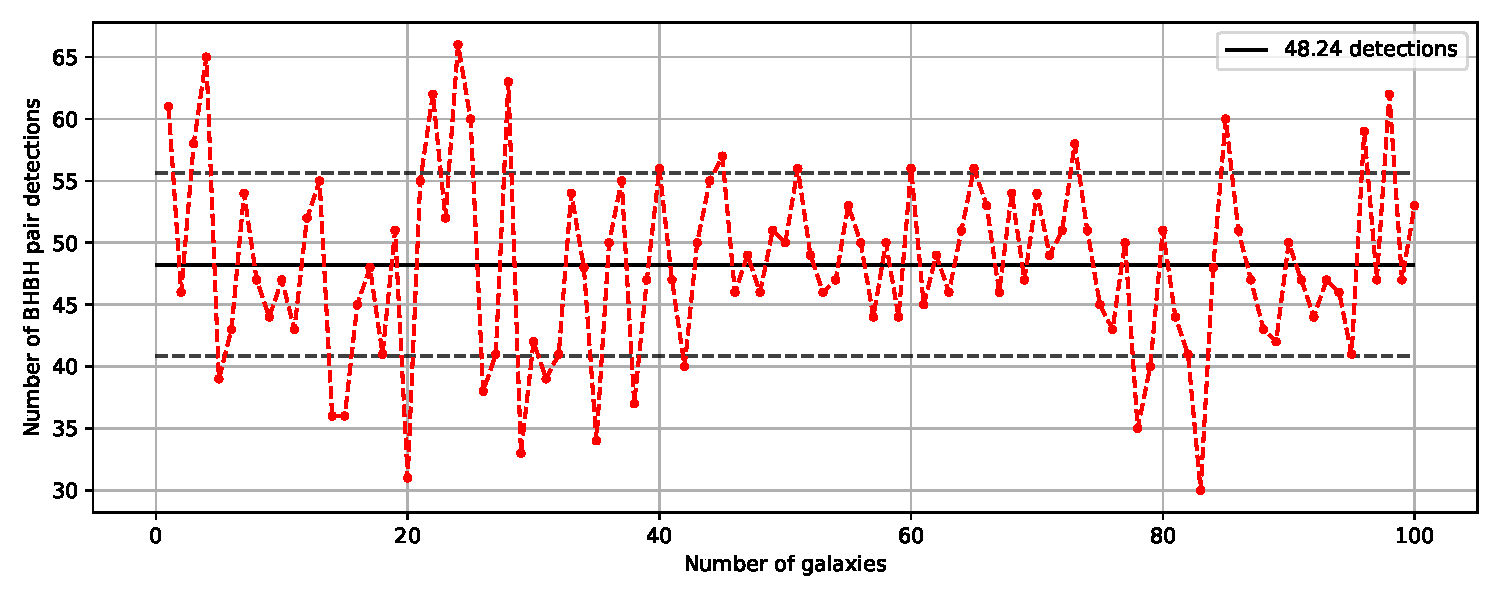
\includegraphics[width=\columnwidth]{analysis_data/main_analysis_folder/BHBH_n_detections}
    \caption{Number of BHBH pair detection per galaxy instance. On average, a total of $\sim$48 pairs per galaxy were detected in this study.}
    \label{fig:bhbhndetections}
\end{figure}

\begin{figure}[!h]
    \centering
    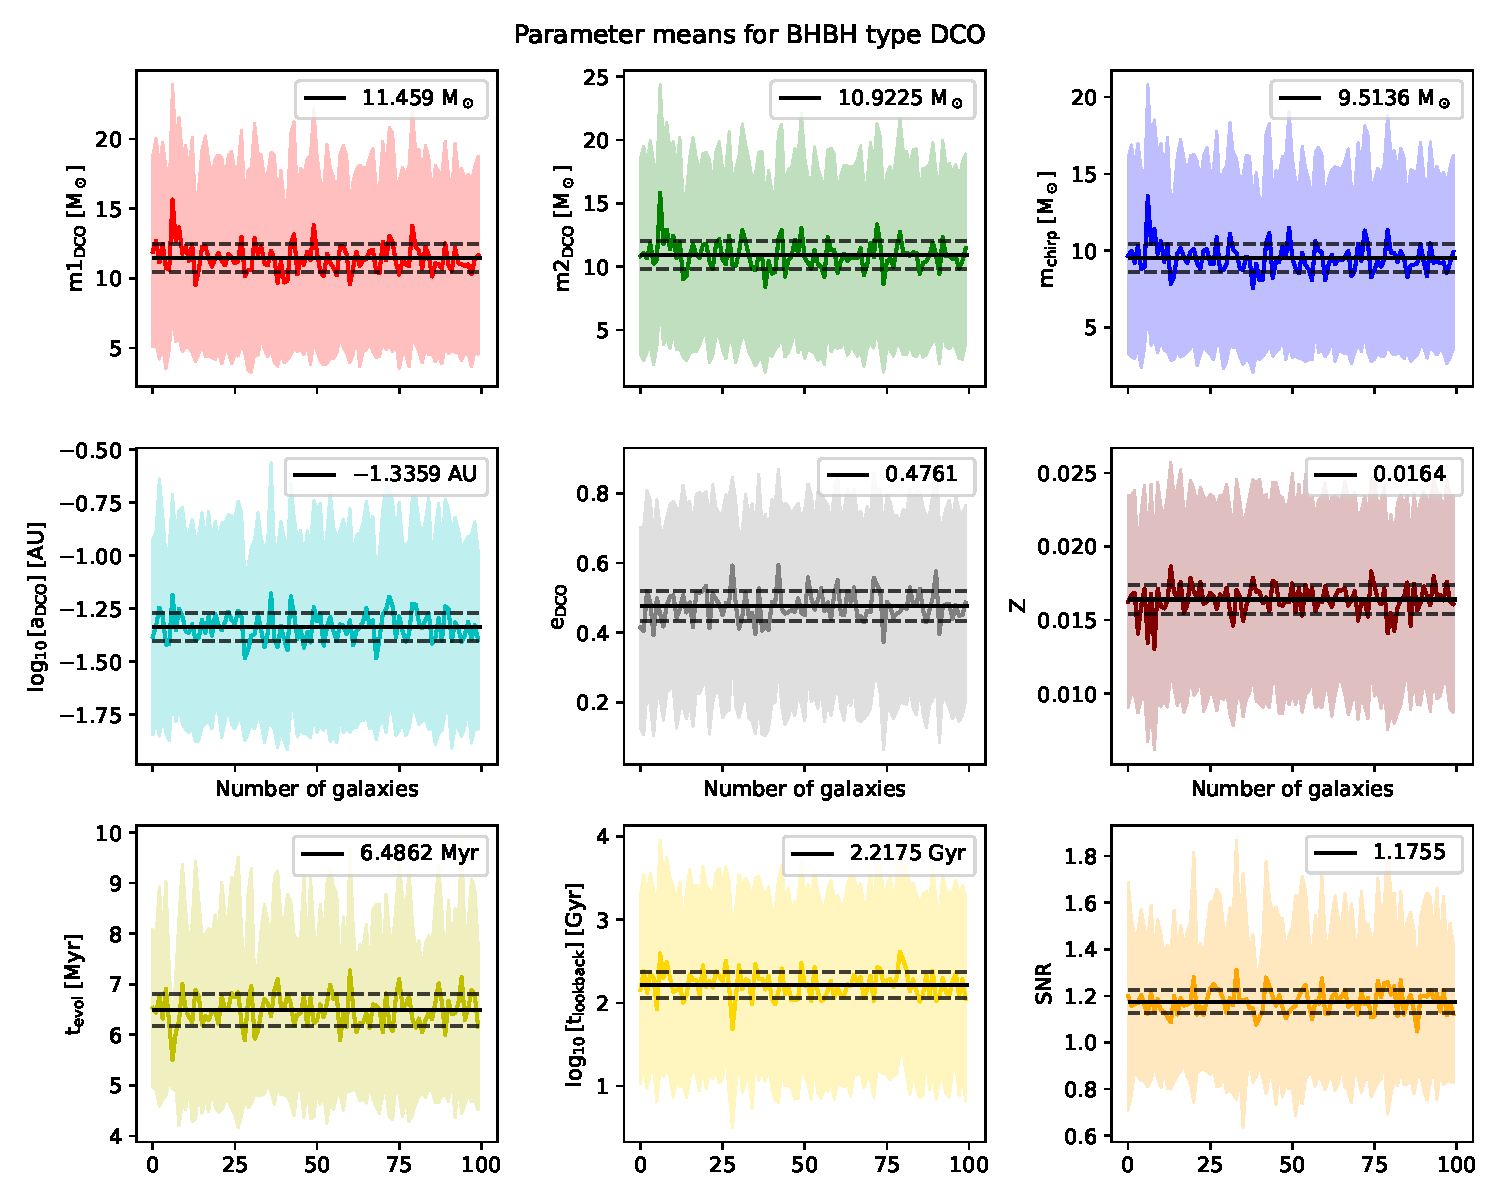
\includegraphics[width=\columnwidth]{analysis_data/main_analysis_folder/BHBH_n_galaxy_mean_plot}
    \caption{The mean and standard deviation for selected parameters in every galaxy, plotted against the galaxy number. An overall measure of mean and standard deviation of all the galaxies is also shown for the selected parameter with a black solid and dashed lines respectively.}
    \label{fig:bhbh_n_galaxy_mean_plot}
\end{figure}

\subsection{Binary Neutron Stars}
\begin{figure}[!h]
	\centering
	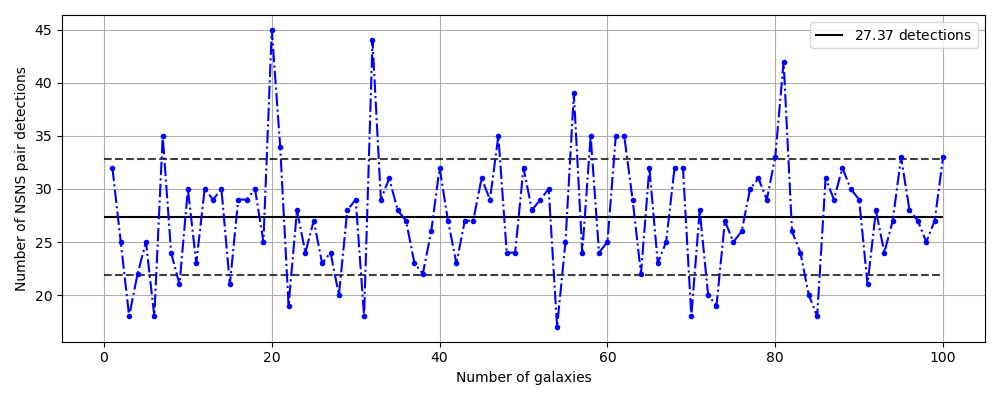
\includegraphics[width=\columnwidth]{analysis_data/main_analysis_folder/NSNS_n_detections}
	\caption{Number of NSNS pair detection per galaxy instance. On average, a total of $\sim$27 pairs per galaxy were detected in this study.}
	\label{fig:nsnsndetections}
\end{figure}

\begin{figure}[!h]
	\centering
	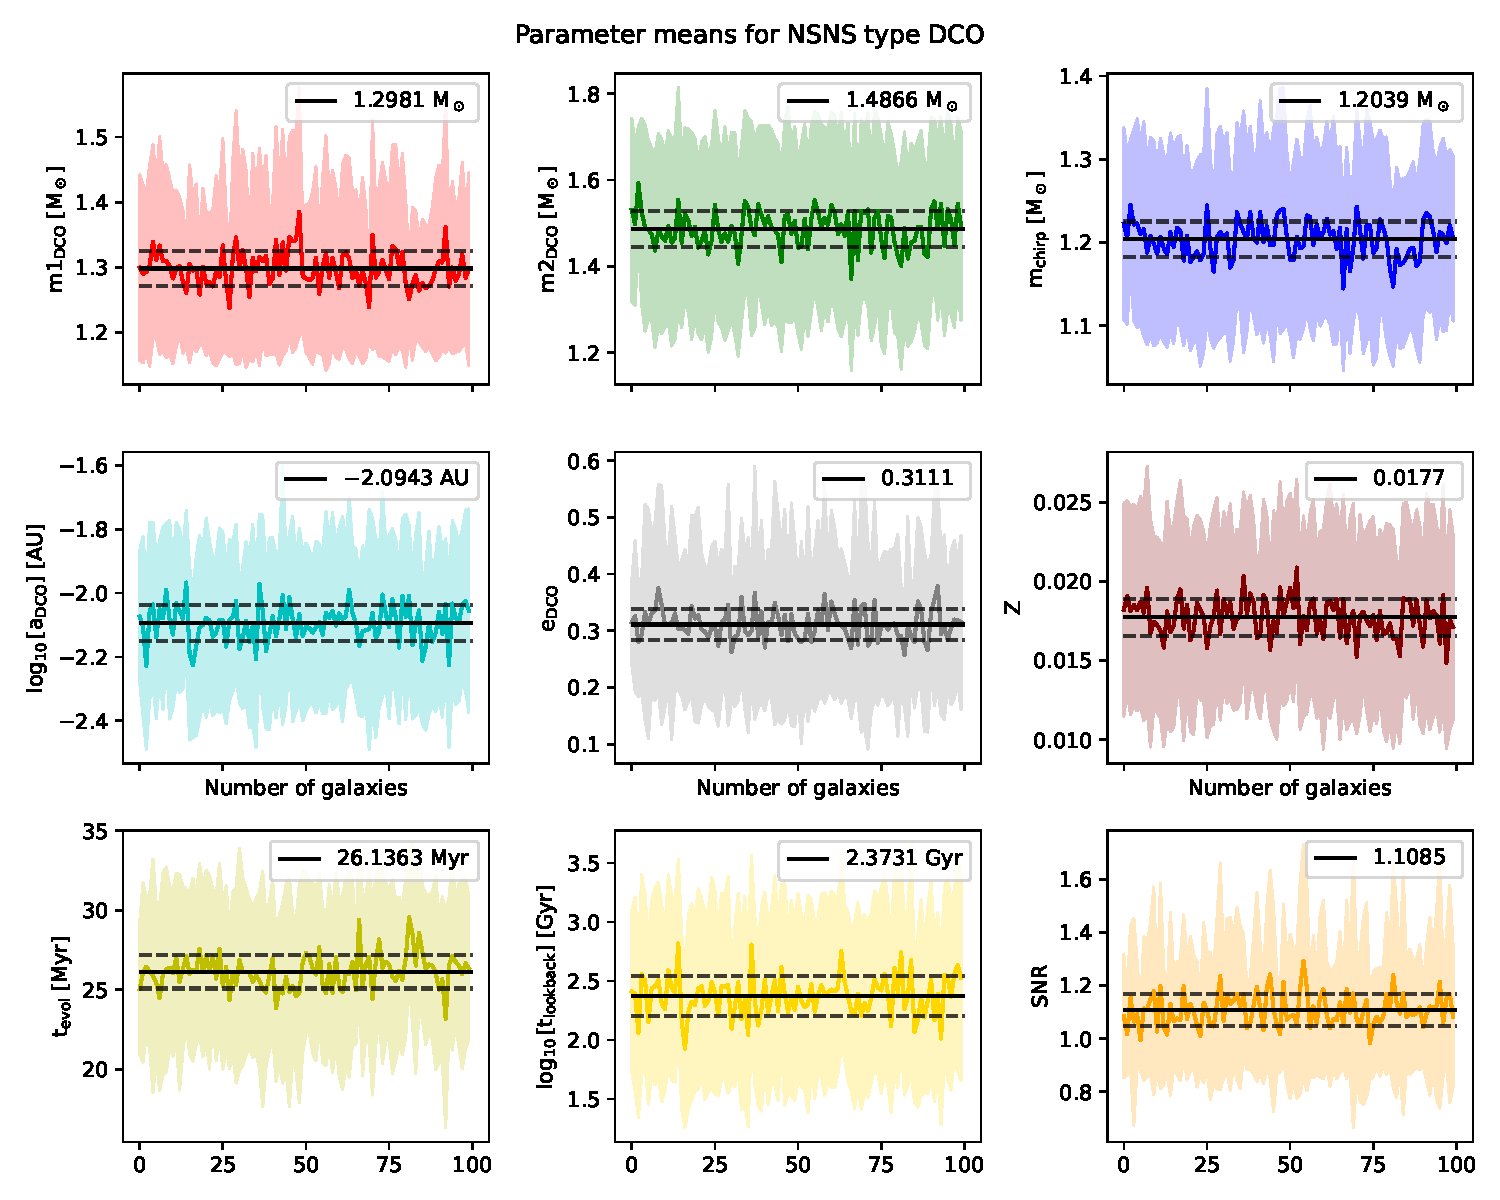
\includegraphics[width=\columnwidth]{analysis_data/main_analysis_folder/NSNS_n_galaxy_mean_plot}
	\caption{Same as figure~\ref{fig:bhbh_n_galaxy_mean_plot}.}
	\label{fig:nsns_n_galaxy_mean_plot}
\end{figure}

\subsection{Neutron Star $-$ Black Hole binary}

\begin{figure}[!h]
	\centering
	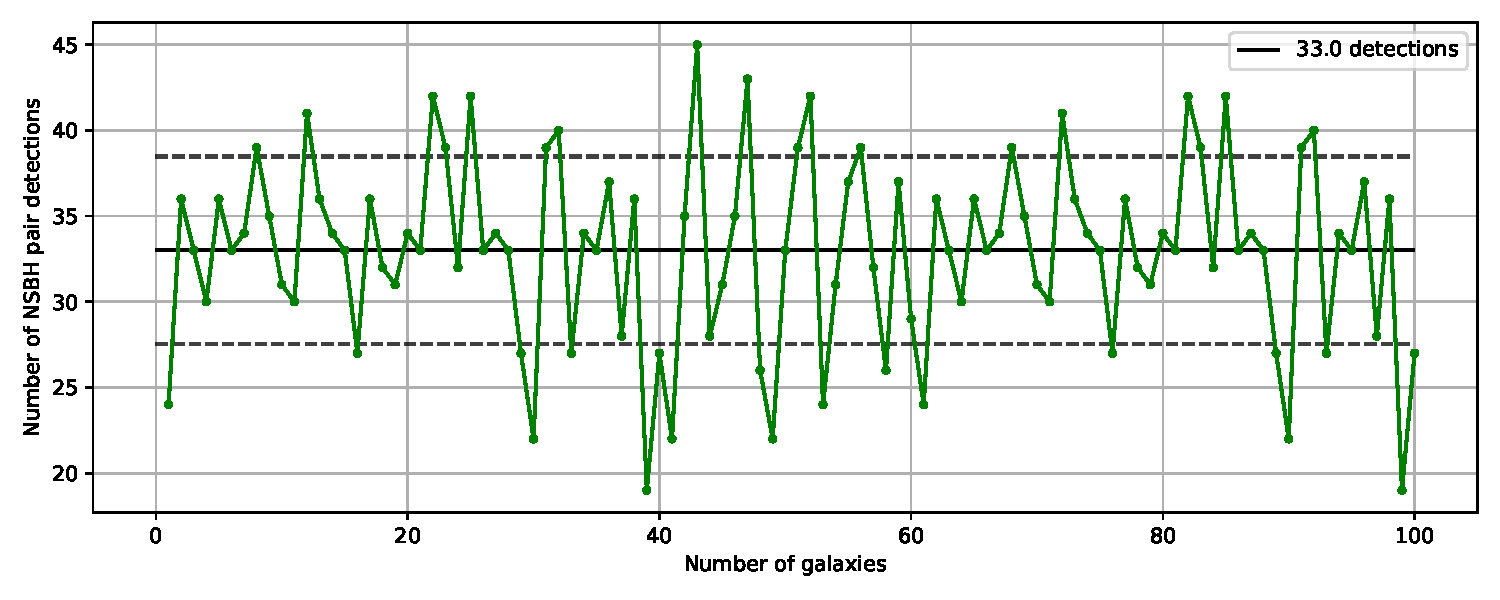
\includegraphics[width=\columnwidth]{analysis_data/main_analysis_folder/NSBH_n_detections}
	\caption{Number of NSBH pair detection per galaxy instance. On average, a total of $\sim$33 pairs per galaxy were detected in this study.}
	\label{fig:nsbhndetections}
\end{figure}	

\begin{figure}[!h]
	\centering
	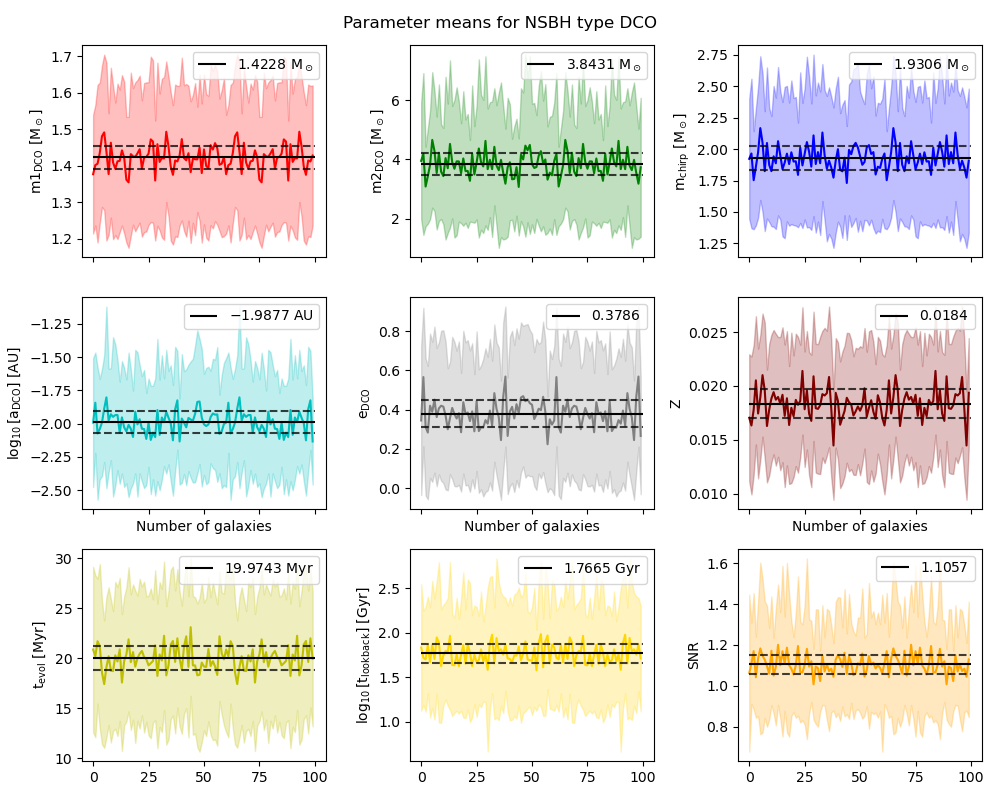
\includegraphics[width=\columnwidth]{analysis_data/main_analysis_folder/NSBH_n_galaxy_mean_plot}
	\caption{Same as figure~\ref{fig:bhbh_n_galaxy_mean_plot}.}
	\label{fig:nsbh_n_galaxy_mean_plot}
\end{figure}

\newpage
\subsection{Black Hole $-$ Neutron Star binary}
\begin{figure}[!h]
	\centering
	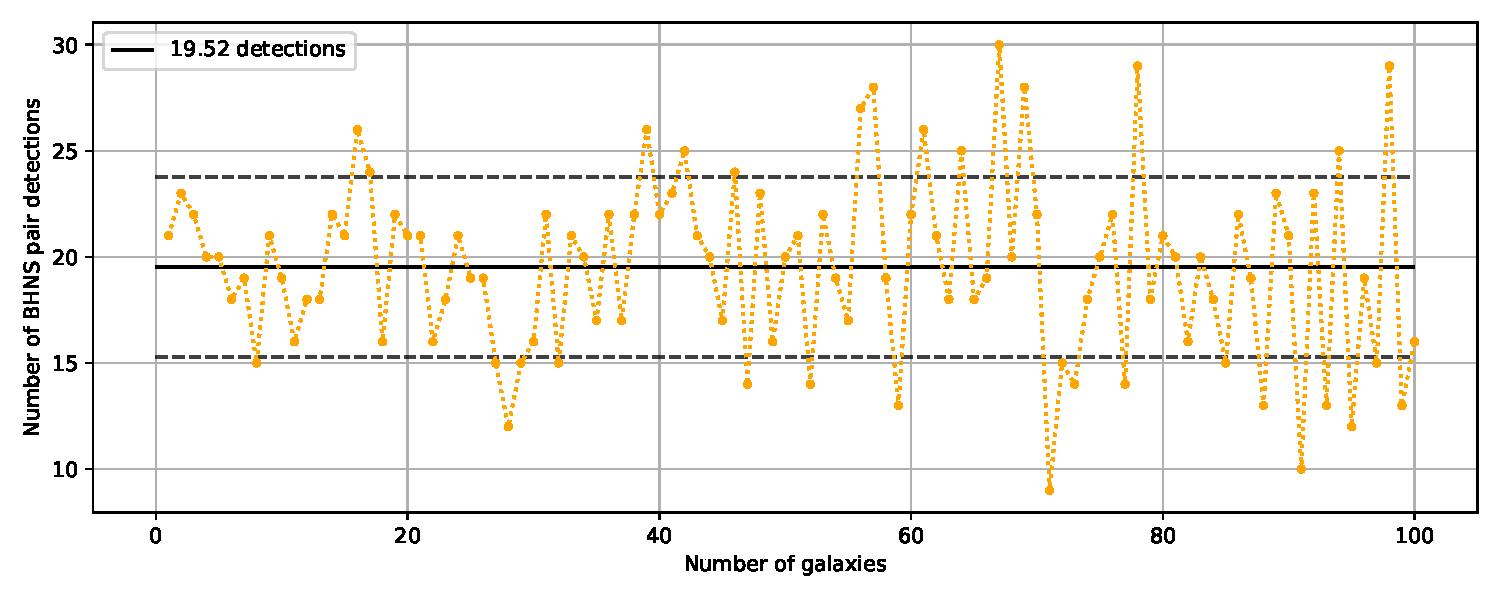
\includegraphics[width=\columnwidth]{analysis_data/main_analysis_folder/BHNS_n_detections}
	\caption{Number of BHNS pair detection per galaxy instance. On average, a total of $\sim$20 pairs per galaxy were detected in this study.}
	\label{fig:bhnsndetections}
\end{figure}	

\begin{figure}[!h]
	\centering
	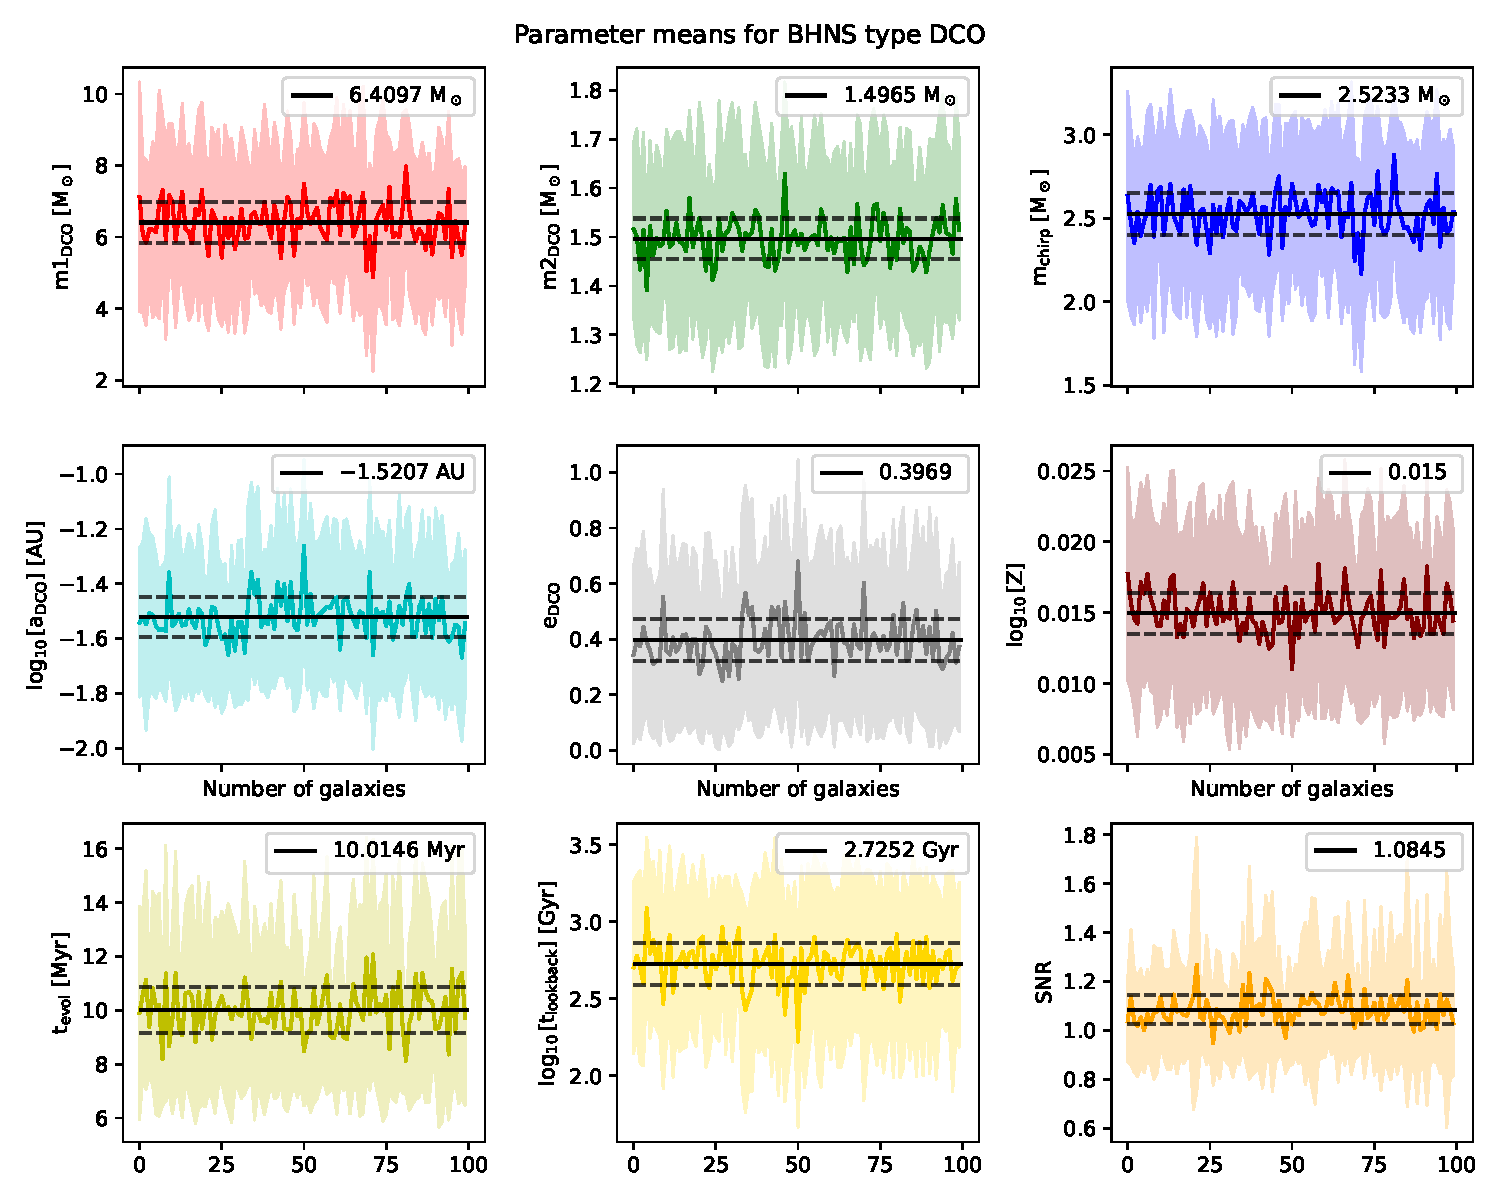
\includegraphics[width=\columnwidth]{analysis_data/main_analysis_folder/BHNS_n_galaxy_mean_plot}
	\caption{Same as figure~\ref{fig:bhbh_n_galaxy_mean_plot}.}
	\label{fig:bhns_n_galaxy_mean_plot}
\end{figure}
